%% LyX 2.3.6.2 created this file.  For more info, see http://www.lyx.org/.
%% Do not edit unless you really know what you are doing.
\documentclass[twocolumn,conference]{IEEEtran}
\usepackage[T1]{fontenc}
\usepackage[latin9]{inputenc}
\usepackage{verbatim}
\usepackage{textcomp}
\usepackage{graphicx}
\usepackage[unicode=true,
 bookmarks=true,bookmarksnumbered=true,bookmarksopen=true,bookmarksopenlevel=1,
 breaklinks=false,pdfborder={0 0 0},pdfborderstyle={},backref=false,colorlinks=false]
 {hyperref}
\hypersetup{pdftitle={Your Title},
 pdfauthor={Your Name},
 pdfpagelayout=OneColumn, pdfnewwindow=true, pdfstartview=XYZ, plainpages=false}

\makeatletter
%%%%%%%%%%%%%%%%%%%%%%%%%%%%%% User specified LaTeX commands.
% for subfigures/subtables
\usepackage[caption=false,font=footnotesize]{subfig}
\usepackage{hyperref}
\hypersetup{colorlinks=true}

\@ifundefined{showcaptionsetup}{}{%
 \PassOptionsToPackage{caption=false}{subfig}}
\usepackage{subfig}
\makeatother

\begin{document}
\title{\texttt{BraggHLS}}
\author{\IEEEauthorblockN{Maksim~Levental}\IEEEauthorblockA{University of Chicago\\
Email: test@test.tes}\and \IEEEauthorblockN{Ryan~Chard}\IEEEauthorblockA{Ecole Superieure\\
Nantes, France\\
Email: second@second.fr}\and \IEEEauthorblockN{Kyle~Chard\\
and Ian~Foster}\IEEEauthorblockA{Star Academy\\
San Francisco, California 99999-9999\\
Telephone: (800) 555\textendash 5555\\
Fax: (888) 555\textendash 5555}}
\maketitle
\begin{abstract}
In many experiment-driven scientific domains, such as high-energy
physics, material science, and cosmology, very high data rate experiments
impose hard constraints on the corresponding data acquisition systems:
collected data must either be indiscriminately stored for post-processing
and analysis, thereby necessitating large storage capacity, or accurately
filtered in real-time, thereby necessitating low latency execution.
Deep neural networks, effective in many other filtering tasks, have
not been widely employed in such data acquisition systems, due to
design and deployment difficulties. This paper presents an open source,
lightweight, compiler framework \texttt{BraggHLS}, based on high-level
synthesis techniques, for translating high-level representations of
deep neural networks to low-level representations, suitable for deployment
to near-sensor devices such as field-programmable gate arrays. We
present a case study and evaluation of \texttt{BraggHLS} on a deep
neural network for Bragg peak detection in the context of high-energy
diffraction microscopy. We show \texttt{BraggHLS} is able to produce
an implementation with a throughput 4.7\textmu s/sample, which is
approximately a 5x improvement over the existing implementation.

\tableofcontents{}
\end{abstract}


\section{Introduction}

Very high data rates are observed and, consequently, large datasets
are generated across a broad range of experiments in scientific domains,
such as high-energy physics, material science, and cosmology. For
example, in high-energy physics, the LHCb detector, at the CERN Large
Hadron Collider, is tasked with observing the trajectories of particles
produced in proton-proton collisions at a rate of 40 million per second
(i.e., 40 MHz) \cite{pmlr-v42-glig14}. With a packet size of approximately
50kB (per collision), this implies a data rate of approximately 2TB/s.
Ultimately, in combination with other detectors, the LHC processes
approximately 100EB of data a year. In materials science, high-energy
diffraction microscopy (HEDM) techniques, which provide non-destructive
characterization of structure and its evolution in a broad class of
single-crystal and polycrystalline materials, can have collection
rates approaching 1 MHz \cite{Hammer_2021}, with a corresponding
packet size of 80kB. In cosmology, the Square Kilometre Array, a radio
telescope projected to be completed in 2024 and to be operational
by 2027 \cite{mcmullin2022square}, will sustain data rates in excess
of 10 TB/s \cite{grainge2017square}.

Naturally, for high data rate experiments, directly storing and distributing
such large quantities of data to the associated research communities
for further analysis is cost prohibitive. Thus, either compression
(in the case of storage and transmission) or outright filtering is
necessary, i.e., only a small fraction of the most ``interesting''
data is selected at time of collection, with the remainder being permanently
discarded. In this work we focus on the filtering approach. Note,
that the tradeoff made in employing filtering should be clear: reduced
storage at the expense of more stringent latency constraints (on the
filtering mechanisms). In addition, the risk of discarding meaningful
data introduces accuracy (of the filtering mechanisms) as a critical
new dimension of the data acquisition systems. Typically, these filtering
mechanisms consist either of physics based models \cite{LHCB-FIGURE-2020-018}
or machine learning models \cite{Gligorov_2013}; in either case maximally
efficient and effective use of the target hardware platform is tantamount
to accuracy. Irrespective of the type of technique employed, almost
universally, for the ultra-low latency use cases (e.g., sub-microsecond
latency constraints), the implementation is deployed to either field-programmable
gate arrays (FPGAs) or application-specific integrated circuits (ASICs)
\cite{Duarte_2018}. %
\begin{comment}
The reason for this is only FPGAs and ASICs are flexible enough to
satisfy the latency constraints for a wide range of techniques. Note,
in this work we focus exclusively on FPGAs.
\end{comment}

Deep neural networks (DNNs), a particular type of machine learning
model, have been shown to be effective in many scientific and commercial
domains due to their ``representational capacity'', i.e., they demonstrate
a capacity to (approximately) represent diverse sets of mappings \cite{alzubaidi2021review}.
DNNs ``learn'' to represent a mapping over the course of ``training'',
wherein they are iteratively evaluated on sample data while a ``learning
rule'' periodically updates the parameters (\emph{weights}) that
parameterize the DNN. In recent years they have been investigated
for near real-time scientific use cases \cite{liu2019deep,patton2018167,liu2022exploring}
but their use for the lowest latency use cases has been very limited
\cite{Duarte_2018}. The reasons for this are threefold: 
\begin{enumerate}
\item Graphics Processing Units (GPUs), the conventional hardware target
for DNNs, until very recently, have not been performant enough for
these very high data rate, very low latency, use cases (due to their
low clock speeds and low peripheral bandwidth \cite{aaij2020allen});
\item DNNs, by virtue of their depth, are resource intensive, in terms of
both memory (for the weights) and compute (floating point arithmetic),
thereby preventing their deployment to FPGAs, which, in particular,
have limited static RAM available;
\item DNNs are (typically) defined, trained, and distributed using high-level
frameworks (such as PyTorch \cite{paszke2017automatic}, TensorFlow
\cite{https://doi.org/10.48550/arxiv.1603.04467}, MXNet \cite{https://doi.org/10.48550/arxiv.1512.01274}),
which abstract all implementation details from the user, thereby making
portability of existing model architectures (to e.g., FPGA) nigh impossible.
\end{enumerate}
These three barriers demand of a solution that can simultaneously
translate a high-level representation of a DNN to a low-level representation,
suitable for deployment to FPGA, while optimizing resource usage and
minimizing latency. In general, the task of \emph{lowering} high-level
representations of programs to lower-level representations is the
domain of a compiler. Similarly, the task of \emph{synthesizing} a\emph{
register-transfer level} (RTL) \emph{design}, rendered in a \emph{hardware
description language} (HDL), from a program, is the domain of high-level
synthesis (HLS) \cite{7368920}. While several such HLS tools exist
\cite{10.1145/2514740,Zhang2008,ferrandi2021bambu} and despite, often,
bundling robust optimizing compilers, they struggle to effectively
perform the necessary optimizations in reasonable amounts of time
(see Section \ref{sec:Evaluation}).

Recently, deep learning compilers (such as TVM \cite{chen2018tvm},
MLIR \cite{https://doi.org/10.48550/arxiv.2002.11054}, and Glow \cite{https://doi.org/10.48550/arxiv.1805.00907})
have demonstrated the ability to dramatically reduce inference latencies
\cite{https://doi.org/10.48550/arxiv.1809.02697}, training times
\cite{9664259}, and memory usage \cite{https://doi.org/10.48550/arxiv.1604.06174}
of DNNs. These compilers function by extracting intermediate-level
representations (IRs) of the DNNs, from the representations produced
by the frameworks, and performing various optimizations on those IRs
(such as kernel fusion \cite{10.1145/2858788.2688521}, vectorization
\cite{maleki2011evaluation}, and memory planning \cite{https://doi.org/10.48550/arxiv.1604.06174}).
The highly optimized IR is then used to generate code for various
target hardware platforms. Given the successes of these compilers,
it's natural to wonder whether they can adapted to the task of sufficiently
optimizing a DNN such that it might be synthesized to RTL, for deployment
to FPGA.

In this paper, we present \texttt{BraggHLS}, an open source, lightweight,
compiler and HLS framework which can lower DNNs defined as PyTorch
models to FPGA implementations. \texttt{BraggHLS} uses a combination
of compiler and HLS techniques to compile the entire DNN into a \emph{statically
scheduled} circuit, thereby eliminating all synchronization overheads
and achieving ultra-low latency. \texttt{BraggHLS} is general and
supports a wide range of DNN layer types, and thus a wide range of
DNNs, but we evaluate it on a DNN designed for identifying Bragg diffraction
peaks. In summary our specific contributions include:
\begin{enumerate}
\item We discuss the challenges faced by a compiler and HLS tool in attempting
to lower DNNs to ultra-low latency designs, including runtime costs
incurred during design space exploration, challenges meeting resource
and timing constraints during synthesis, placement, and routing;
\item We describe and implement a compiler framework, \texttt{BraggHLS},
which can effectively transform unoptimized, hardware-agnostic PyTorch
models into ultra-low latency RTL designs suitable for deployment
to Xilinx FPGAs. \texttt{BraggHLS} is thoroughly tested, open source,
and available at \href{https://github.com/makslevental/bragghls/}{https://github.com/makslevental/bragghls/};
\item We show that designs generated by \texttt{BraggHLS} achieve lower
latency than Xilinx's state-of-the-art commercial HLS tool (Vitis
HLS) for a variety of DNN layer types. In particular we show that
\texttt{BraggHLS} can produce synthesizable designs that meet placement,
routing, and timing constraints, where Vitis HLS cannot.
\end{enumerate}
The rest of this paper is organized as follows: Section \ref{sec:Background}
reviews key concepts from compilers, high-level synthesis, and FPGA
design flows. Section \ref{sec:BraggHLS-compiler-and} describes the
\texttt{BraggHLS} compiler and HLS framework in detail. Section \ref{sec:Evaluation}
describes \texttt{BraggNN}, the Bragg peak detection DNN, and evaluates
\texttt{BraggHLS}\textquoteright s resource efficiency, scalability,
and competitiveness with designs generated by Vitis HLS. Finally,
Section \ref{sec:Conclusion} concludes with a summary, and related
and future work.

\section{Background\label{sec:Background}}

\subsection{Compilers: the path from high to low}

The path from a high-level, abstract, representations of a DNN to
a register-transfer level representation can be neatly formulated
as a series of progressive lowerings between adjacent levels of abstraction.
Each level of abstraction is rendered as a programming language, IR,
or HDL and thus we descibe each lowering in terms these representations
and the tools that manipulate them:
\begin{enumerate}
\item An imperative, \emph{define-by-run,} Python representation, in PyTorch;
\item High-level data-flow graph representation, in TorchScript;
\item Low-level data and control flow graph representation, in MLIR.
\end{enumerate}
%

\subsubsection{PyTorch and TorchScript}

Typically DNN models are represented in terms of high-level frameworks,
themselves implemented within general purpose programming languages.
Such frameworks are widely used because of their ease of use and large
library of example implementations of various DNN model architectures.
Since \texttt{BraggNN} is implemented using PyTorch, we focus on relevant
aspects of PyTorch. DNNs developed within PyTorch are \emph{defined-by-run}:
the author imperatively describes the DNN in terms of high-level operations,
using python, which when executed materializes the high-level data-flow
graph (DFG) corresponding to the DNN (e.g., for the purposes of reverse-mode
automatic differentiation). From the perspective of the user, define-by-run
enables fast iteration at development time, possibly at the cost of
some runtime performance. 

From the perspective of compilation, define-by-run precludes efficient
extraction of the high-level DFG; since the DFG is materialized only
at runtime, it cannot be inferred from the textual representation
(i.e., the python source) of the DNN. Furthermore, apriori, the runtime-materialized
DFG is only partially materialized\footnote{``...instead, every intermediate result records only the subset of
the computation graph that was relevant to their computation.'' \cite{paszke2017automatic}}, and only as an in-memory data structure. Thus, framework support
is necessary. Indeed, PyTorch supports a Single Static Assignment
(SSA) IR, called TorchScript (TS) IR and accompanying tracing mechanism
(the TS JIT) to produce TS IR from conventionally defined PyTorch
models. Lowering from PyTorch to TS IR enables various useful analyses
and transformations on a DNN at the level of the high-level DFG (such
as kernel fusion \cite{10.1145/2858788.2688521}) but targeting FPGAs
requires a broader collection of transformations. To this end, we
turn to a recent addition to the compiler ecosystem.

\subsubsection{MLIR}

Multi-level Intermediate Representation \cite{https://doi.org/10.48550/arxiv.2002.11054}
presents a new approach to building reusable and extensible compiler
infrastructure. MLIR is composed of a set of \emph{dialect} IRs, subsets
of which are mutually compatible, either outright or by way of translation/legalization.
The various dialects aim to capture and formalize the semantics of
compute intensive programs at varying levels of abstraction, as well
as namespace related sets of IR transformations. The entrypoint into
this compiler framework, from PyTorch, is the \texttt{torch} dialect
\cite{torch-mlir}, a high-fidelity mapping from TS IR to MLIR native
IR, which, in addition to performing the translation to MLIR, fully
refines all shapes of intermediate tensors in the DNN (i.e., computes
concrete values for all dimensions of each tensor); this is necessary
for downstream optimizations and eliminating inconsistencies \cite{https://doi.org/10.48550/arxiv.2203.08402}.

While the \texttt{torch} dialect is necessary for lowering to MLIR
and shape refinement, it is a representation of a DNN at the same
level of abstraction as TS IR: it does not capture the precise data
flow and control flow necessary for novel implementations of DNN operations
(e.g., for FPGA). Fortunately, MLIR supports lower-level dialects,
such as the \texttt{affine} and \texttt{scf} (structured control flow)
dialects. The \texttt{scf} is a straightforward formalization of control
flow primitives, such as conditionals and loops, so we do not discuss
it in great detail. The \texttt{affine} dialect, on the otherhand,
provides a formalization of semantics that lend themselves to polyhedral
compilation techniques \cite{polyhedral-mlir}, i.e., techniques that
make dependence analysis and loop transformations efficient and reliable.
We discuss the importance of loop transformations in Section \ref{sec:BraggHLS-compiler-and}.

\subsection{High-level synthesis and FPGA design}

\subsubsection{High-level synthesis}

High-level synthesis tools produce RTL descriptions of digital designs
from high-level representations, such as C or C++ \cite{10.1145/2514740,ferrandi2021bambu}
or LLVM IR. In particular, Xilinx's Vitis HLS, based on the Autopilot
project \cite{Zhang2008}, recently enabled passing LLVM IR to the
tool, rather than C/C++. Given a high-level, procedural, representation,
HLS proceeds in three steps, in order to produce a corresponding RTL
design:
\begin{enumerate}
\item HLS schedules operations (such as \texttt{fmul}, \texttt{fadd}, \texttt{load},
\texttt{store}) in order to determine which operations should occur
during each clock-cycle. Such a schedule depends on three characteristics
of the high-level representation:
\begin{enumerate}
\item The topological ordering of the DFG/CFG of the procedural representation
(i.e., the dependencies of operations on results of other operations
and resources);
\item The completion time for each operation;
\item The user's desired clock rate/frequency;
\end{enumerate}
\item HLS associates operations to particular RTL instantiations (called
\emph{binding}) for those operations; for example whether to associate
an add operation followed by a multiply operation to two separate
instances, or whether to associate them both with a single instance
(e.g., configured to perform a fused-multiply-add);
\item HLS builds an finite-state machine (FSM) that functions as control
logic for the sequence of operations in the schedule.
\end{enumerate}
In addition to fulfilling these three fundamental tasks, high-level
synthesis tools such perform standard compiler optimization passes
on the IR (that they ingest or produce internally). Optimization passes
such as store-load forwarding, common subexpression elimination, and
constant propagation, loop-unrolling and tiling. Note that these optimization
passes exhibit varying levels of runtime complexity, e.g., store-load
forwarding in combination with loop-unrolling is polynomial in the
``trip-count'' of the loop nest. Note also that the scheduling problem
solved by HLS is reducible an integer linear programming problem (ILP),
instances of which are NP-hard in general. Thus, HLS tools solve computationally
intensive problems in order to produce a RTL description of a high-level
representation of a DNN. These ``development time'' costs (i.e.,
runtime of the tools) impose practical limitations on the amount of
design space exploration (for the purpose of achieving latency goals)
which can be performed. 

\subsection{FPGA design}

At the RTL level of abstraction, there remain two more steps prior
to being able to actually deploy to an FPGA; one of them being a final
lowering, so called logic synthesis, and the other being place and
route (P\&R). Logic synthesis is the process of mapping RTL to actual
hardware primitives on the FPGA (so-called \emph{technology mapping}),
such as lookup tables (LUTs), block RAMs (BRAMs), flip-flops (FFs),
and digital signal processors (DSPs). Logic synthesis produces a network
list (\emph{netlist}) describing the logical connectivity of various
parts of the design. Logic synthesis effectively determines the implementation
of floating point operations in terms of DSPs; depending on user parameters
and other design features, DSP resource consumption for floating point
multiplication and addition can differ greatly. The number of LUTs
and DSPs that a high-level representation of a DNN corresponds to
is relevant to both the performance and feasibility of that DNN when
deployed to FPGA.

After the netlist has been produced, the entire design undergoes P\&R.
The goal of P\&R is to determine which configurable logic block within
an FPGA should implement each of the units of logic required by the
digital design. P\&R algorithms need to minimize distances between
related units of functionality (in order to minimize wire delay),
balance wire density across the entire fabric of the FPGA (in order
to reduce route congestion), and maximize the clock speed of the design
(a function of both wire delay, logic complexity, and route congestion).
The final, routed design, can then be deployed to the FPGA by producing
a proprietary \emph{bitstream}, which is written to the FPGA.

\section{\texttt{BraggHLS} compiler and HLS framework\label{sec:BraggHLS-compiler-and}}

\section{Evaluation\label{sec:Evaluation}}

asdasd
\begin{figure*}[tbh]
\begin{centering}
\subfloat[\texttt{addmm}]{\centering{}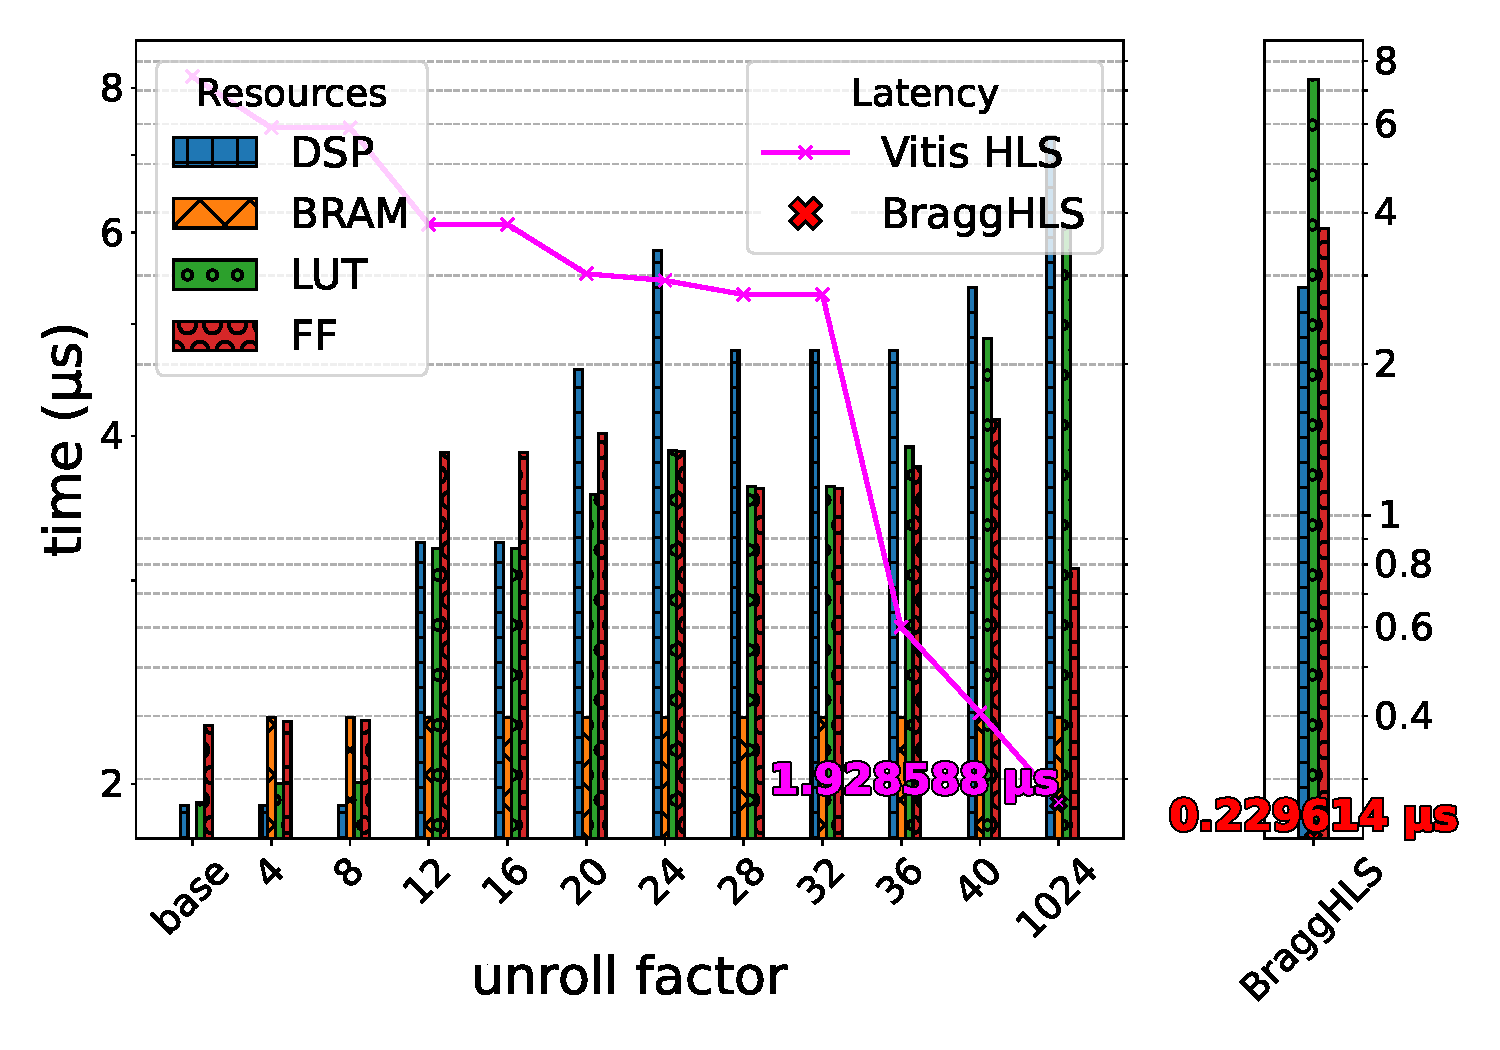
\includegraphics[width=1\columnwidth]{/Users/mlevental/dev_projects/hls_paper/data/cpps/addmm}\label{2dlattice-1-1-2}}\subfloat[\texttt{braggnn}]{\centering{}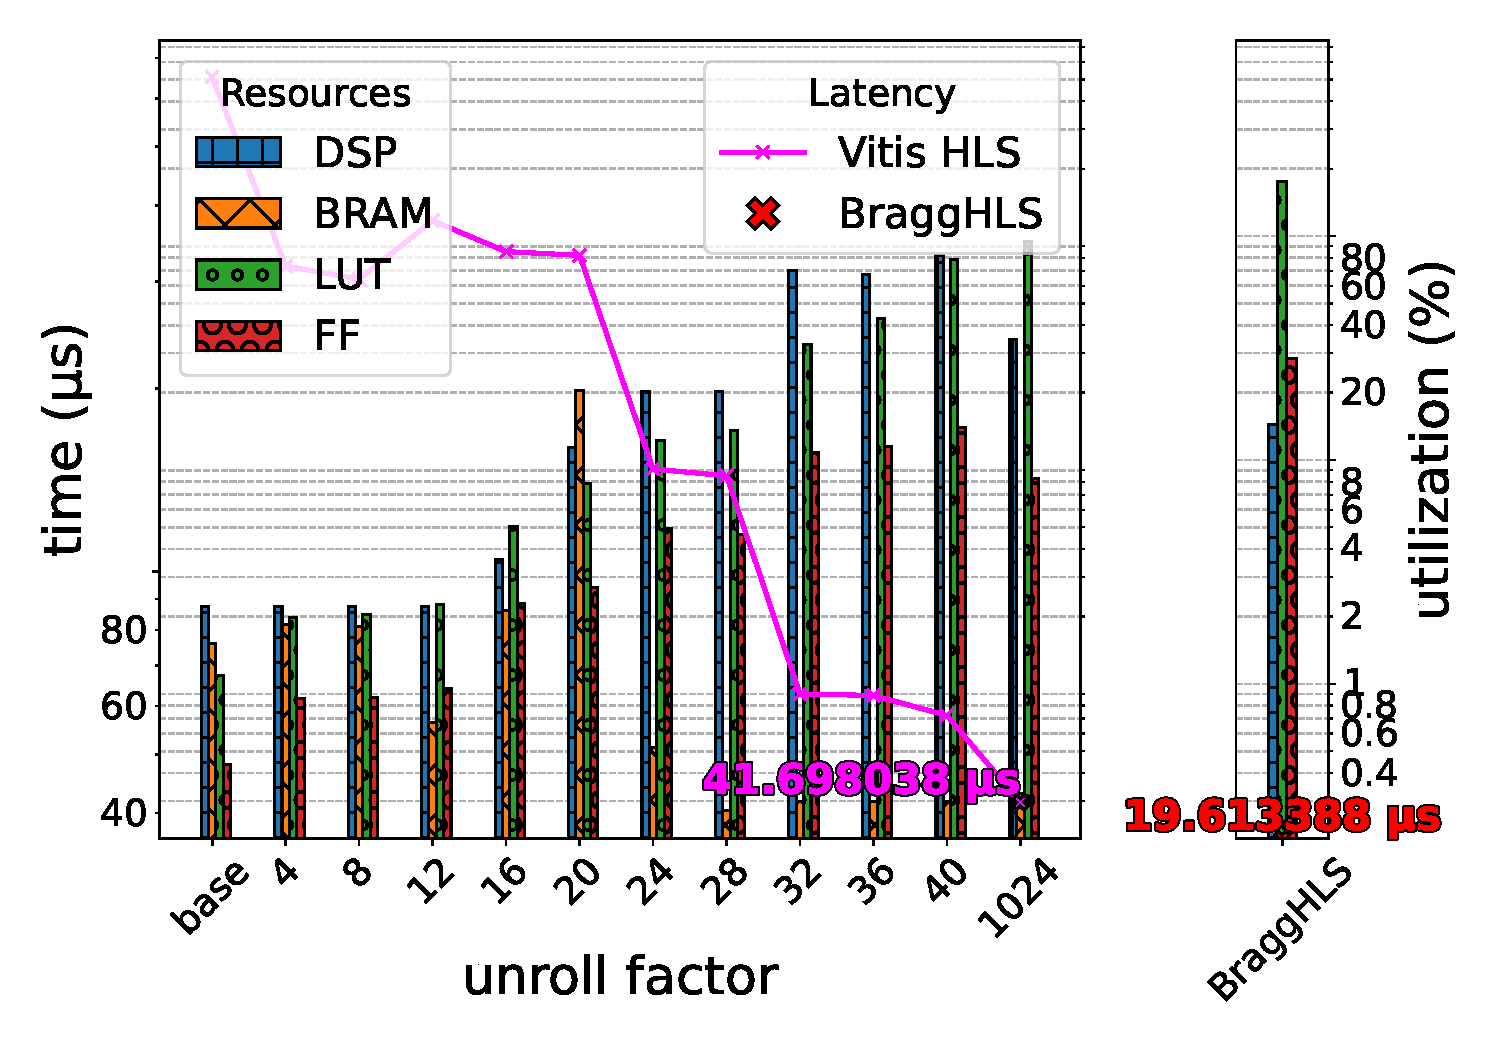
\includegraphics[width=1\columnwidth]{/Users/mlevental/dev_projects/hls_paper/data/cpps/braggnn}\label{2dlattice-1-2-2}}
\par\end{centering}
\medskip{}

\centering{}\label{2dlattice-1-3}\subfloat[\texttt{conv}]{\centering{}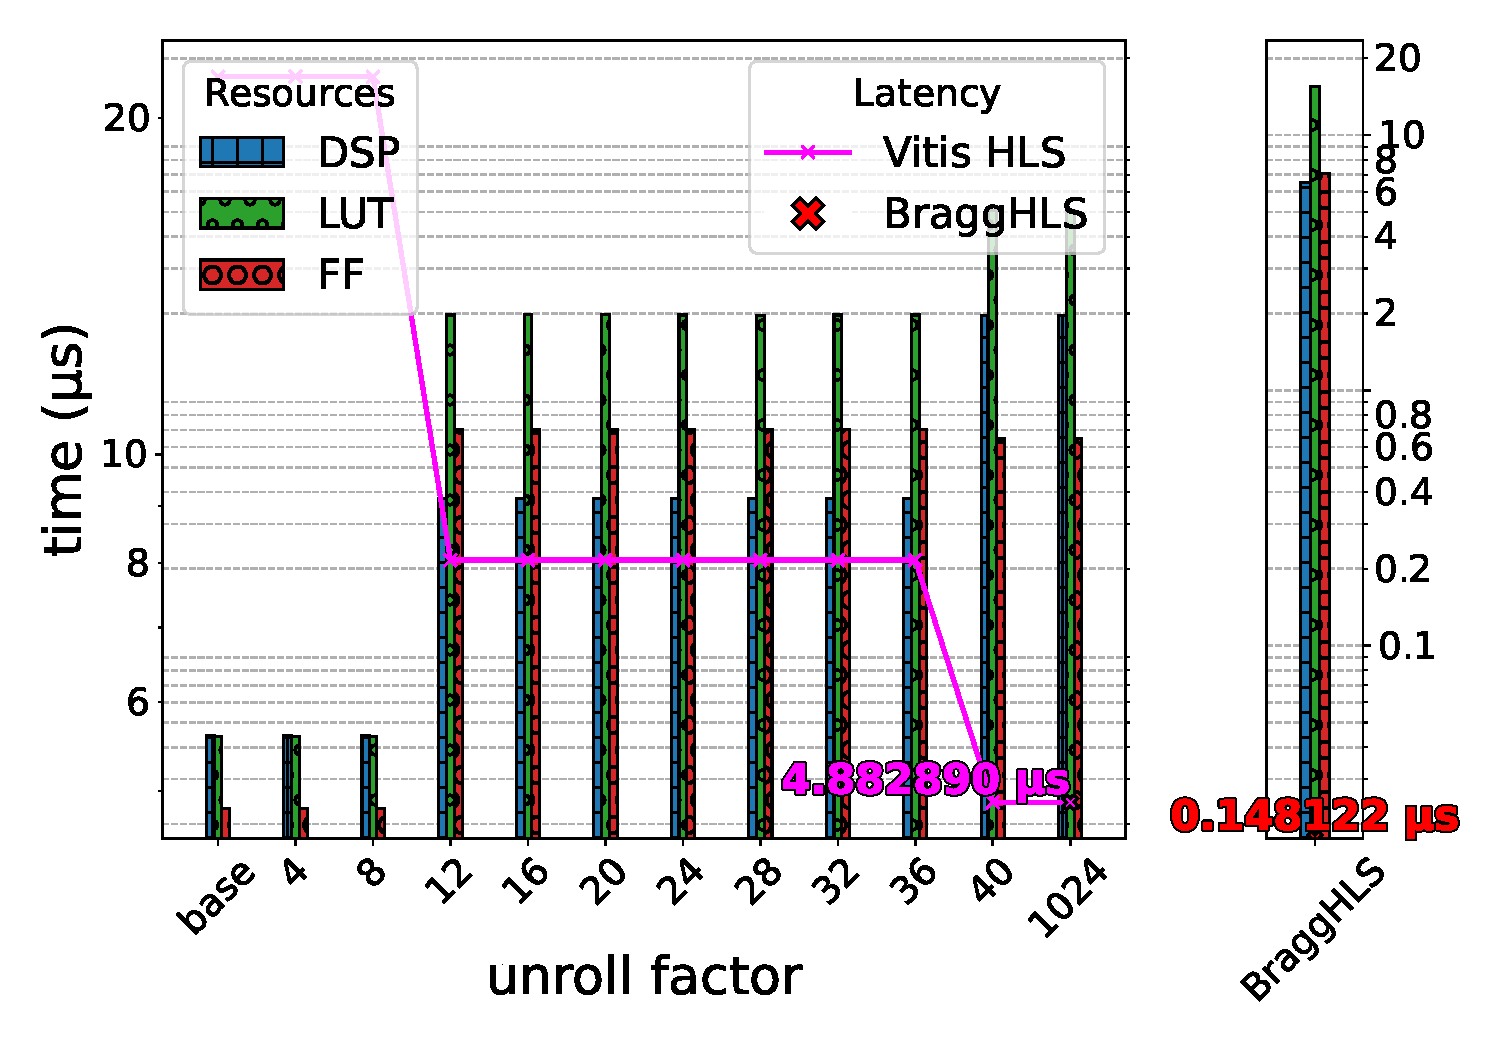
\includegraphics[width=1\columnwidth]{/Users/mlevental/dev_projects/hls_paper/data/cpps/conv}\label{2dlattice-1-1-1-1}}\subfloat[\texttt{matmul}]{\centering{}\includegraphics[width=1\columnwidth]{/Users/mlevental/dev_projects/hls_paper/data/cpps/matmul}\label{2dlattice-1-2-1-1}}\caption{Resource usage and latency vs. unroll factor of various DNN modules.}
\end{figure*}
\begin{figure*}[tbh]
\centering{}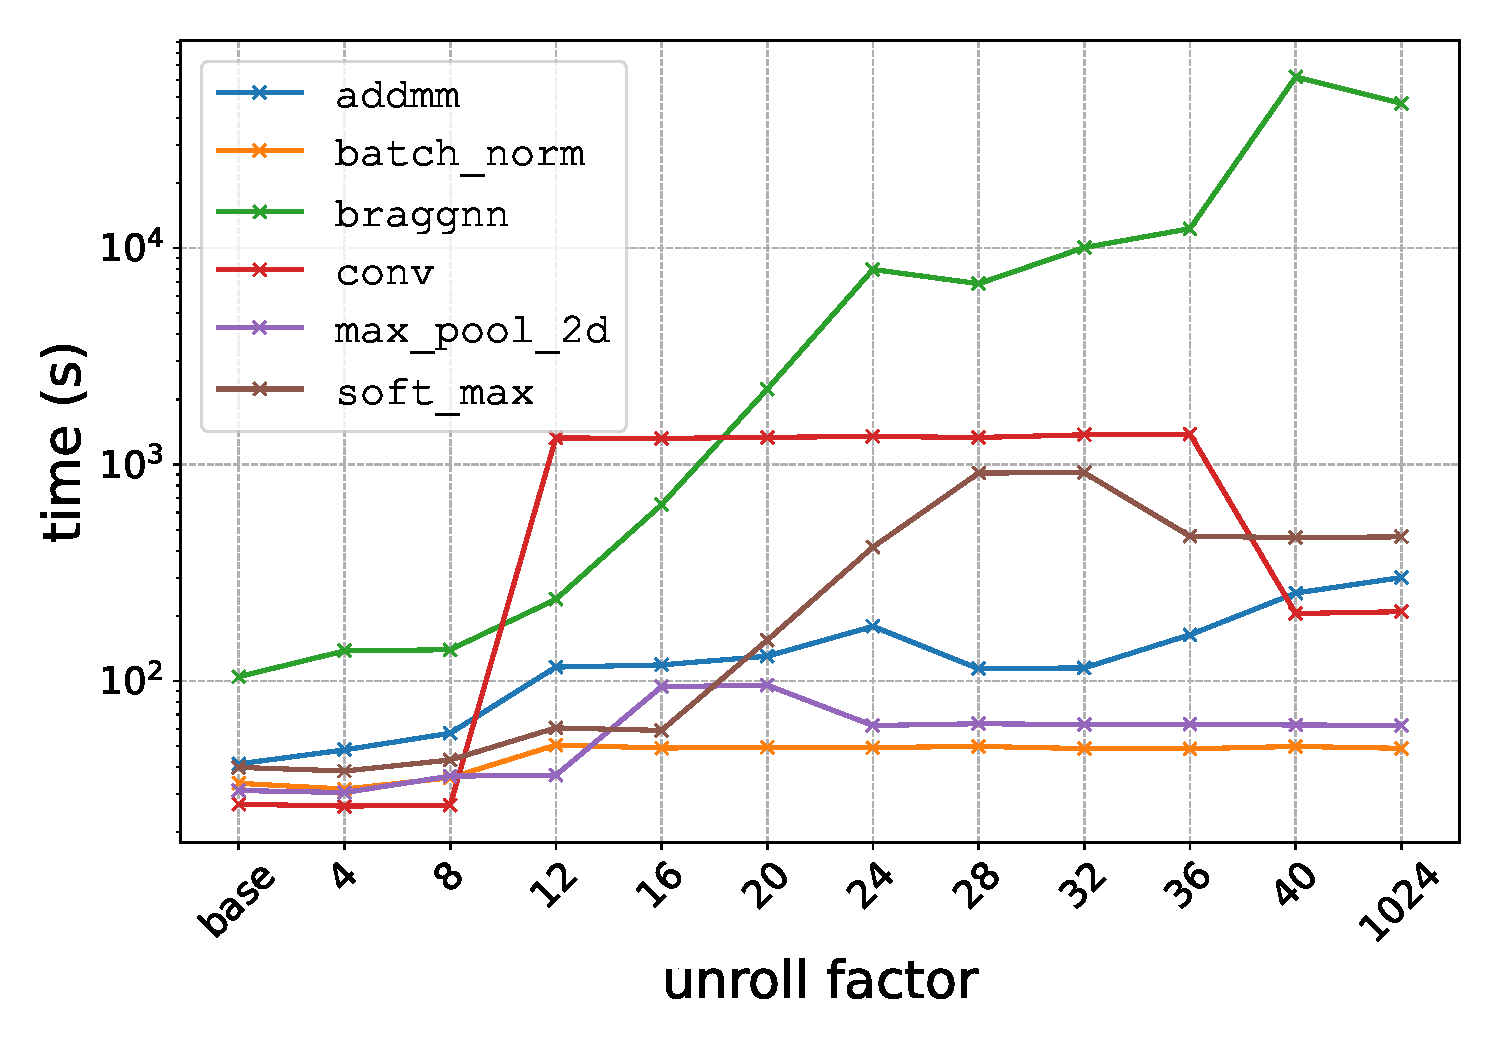
\includegraphics[width=1\columnwidth]{/Users/mlevental/dev_projects/hls_paper/data/cpps/elapsed_time}\caption{Runtime of Vitis HLS vs. unroll factor.}
\end{figure*}


\section{Conclusion\label{sec:Conclusion}}

\bibliographystyle{IEEEtran}
\bibliography{ref}

\end{document}
